% To print single-sided: delete ",twoside" below
\documentclass[11pt,twoside]{article}

% Some very basic packages. Feel free to add your favorites!
\usepackage{amsmath}
\usepackage{amssymb}
\usepackage{amsthm}
\usepackage{upgreek}
\usepackage{fancyhdr}
\usepackage{graphicx}
\usepackage{enumerate}

% Set up the page correctly
\addtolength{\oddsidemargin}{-.54in}
\addtolength{\evensidemargin}{-1.2in}
\addtolength{\textwidth}{1.75in}
\addtolength{\topmargin}{-.875in}
\addtolength{\textheight}{1.75in}
\setlength{\parindent}{0pt}
\setlength{\parskip}{5pt plus 1pt}

% Some nifty commands. Thanks Adam Blank!
\newcommand{\question}[2] {\vspace{.25in} \hrule\vspace{0.5em}
\noindent{{\bf #1:} #2} \vspace{0.5em}
\hrule \vspace{.10in}}
\renewcommand{\part}[1] {\vspace{.10in} {\bf (#1)}}

% Add an image centered on the page.
% The first parameter is a scale factor (set to 1 for no scale)
% The second paramter is the image file. Make sure it is in the same folder as your .tex file!
\newcommand{\centergfx}[2]{\begin{center}\includegraphics[scale = #1]{#2}\end{center}}

% Command to insert a minus sign with a dot over it. Stolen from
% http://www.cs.miami.edu/~burt/learning/Math688.931/Other/errata.tex
\newcommand{\monus}{\stackrel{{}^{\scriptstyle .}}{\smash{-}}}
\newcommand{\bra}[1]{\langle #1 |}
\newcommand{\ket}[1]{| #1 \rangle}
\newcommand{\inner}[2]{\langle #1 | #2 \rangle}
\newcommand{\avg}[1]{\langle #1 \rangle}
\newcommand{\pderiv}[2]{\frac{\partial #1}{\partial #2}}

%%%%%%%%%%%%%%%%%%%%%
%		Replace "Name" and                 %
%		   "andrewid" below                   %
%%%%%%%%%%%%%%%%%%%%%
\newcommand{\myname}{Arjun Kar, Philip Massey}
\newcommand{\myandrew}{(arjunkar, pmassey)}
\newcommand{\mysection}{}
\newcommand{\myhwnum}{}
\newcommand{\myclass}{15-418 Parallel Computer Architecture and Programming}

% Set up the nice header
\pagestyle{fancyplain}
%\chead{\fancyplain{}{ \myname \ \myandrew \ \\ } }
\lhead{\fancyplain{}{ \myname \\ \myandrew \ \\ } \textbf{Final Project Report \myhwnum}}
\rhead{\myclass}
%\rhead{\fancyplain{}{\myclass}}

\begin{document}

\vspace*{0 mm}

\section{Summary}

We implemented a convolutional neural network (LeNet) in Halide, compared correctness with a Theano (Python) implementation, and raced the industry standard neural network software (Caffe) CPU implementation.
We demonstrated that our Halide implementation can achieve performance within 14\% of the baseline Caffe implementation on a 12-core Intel Xeon CPU.

\section{Background}

We will first describe a neural network at a high level, since this concept is crucial to the project.
A neural network, for our purposes, is a machine learning structure that can be drawn as a directed layer graph, where each layer of nodes takes input from the layer below and outputs to the layer above.
We will use this structure to classify images, and the final layer will be a maximum over probabilities of the input to be in a certain class.
Additionally, each ``hidden" node of the network (an interior node that is not located in the bottom-most or top-most layer) performs an activation on the sum of its inputs multiplied by its parameters.
The activation is commonly chosen to be the hyperbolic tangent function, for a reason beyond the scope of this write-up.
We will sometimes refer to these hidden layers as ``convolution" layers, as the size of the weight filter is not generally equal to the size of the image, so we must convolve the input with the weight matrices. 
This is shown in Figure 1, an example neural network.
A neural network is trained by running images through the network, calculating the loss function, and then calculating gradients (for gradient descent) by sending information backward through the network.  
This is commonly known as backpropagation.  
The loss function can be varied, and is not crucial to understand, but essentially respresents how far from the optimal parameters we are.
The backpropagation algorithm uses this loss function (which we only know after evaluating the network on training data) to compute what direction we should change our parameters (i.e. whether to decrease, increase, or remain roughly the same).
This direction (and magnitude) is just the gradient of the loss function with respect to the parameters, which is why the training algorithm for individual nodes is called gradient descent.
As a last point, the Caffe learning framework is currently the industry standard for training and evaluating neural networks; the Theano framework is another that is easier to modify and understand, since it is in Python.

In addition to neural networks, out project involves a domain-specific language known as Halide, developed at MIT.
Here we will give a brief overview of Halide's features.
Halide is a JIT-compiled language for image processing and pipelining that offers high level abstractions for programmers to implement powerful low level optimizations.
Halide splits code into two sections: the first portion of any Halide program defines the algorithm to be executed, and the second portion (optional) defines the schedule on which to execute the algorithm.
Halide algorithms define images via functions by pixel-by-pixel definitions.
These transformative functions take an image and an input and give an image as an output.
We can define a pipeline of these functions in order to transform the input image into the class the network classifies it as.
The scheduling portion of Halide code is where major optimizations such as tiling or parallelizing can be defined.
The image processing abstractions such as tiling, fusing, parallelizing, and others are optimized by Halide's compiler for the particular system on which Halide is being run, which allows development of ultra-portable code that optimizes itself intelligently for a given architecture.

To conclude the background section we will discuss an implementation of LeNet, a certain neural network.
LeNet, named after Yann LeCunn, is made up of two convolution layers (which are also max-pooled, that is to say we subsample the convolved matrix using a simple max function to reduce image size), a fully connected layer (which is simple matrix multiplications of the previous layer's output), and a softmax layer (which actually gives us the predicted class).
LeNet has been proven to work well on the MNIST data set, which is a collection of hand-drawn numbers (from 0 to 9).
The classification task therefore has 10 natural classes, and LeNet has demonstrated $\geq$95\% accuracy on MNIST with just 4 nodes in the first convolution layer and 6 in the second.

\begin{figure}
\centering
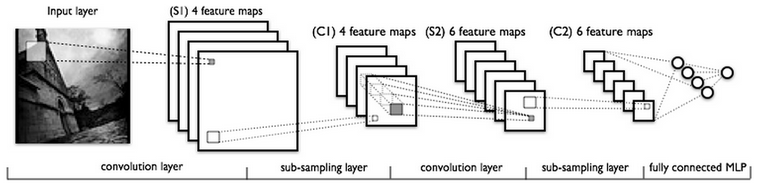
\includegraphics[scale=.8]{network.png}
\caption{Outline of the LeNet neural network.}
\end{figure}

\section{Approach}

Our approach used the Halide language, the Caffe learning framework, the Theano learning framework, and the Latedays cluster.
We used an Intel Xeon 12-core CPU on the Latedays clusters to perform our computation.
In implementing LeNet, we did not need to change the general serial algorithm.
In order to introduce parallelism, we allowed for multiple images to be classified at the same time, and noting portions of the layer computations that could be done simultaneously.
The coding of the algorithm in Halide did not require many iterations, since most of the structure had already been clearly outlined in documentation of LeNet and Theano.

Our implemention of LeNet in Halide started with mapping the concept of neural network layers to Halide semantics.
In order to do this, we need to define the data, which is a Halide image that travels through the neural network, and the layers, which are Halide functions that transform the image as it travels.
The data is a 4D image, where the dimensions are the x and y pixel coordinate, the feature map number, and the image number.
By defining the data as this kind of image, we will be able to exploit many kinds of inherent parallelism, as well as easily perform the matrix operations neccessary for classification.
The layers are Halide functions that take in the data image as input (as well as the weight image, bias image, and other neccessary parameters) an perform a predefined operation on the data.
By defining layers in this way, each layer only needs to perform a simple calculation.
The majority of the layers can represent their operation in one line of Halide code, as the inclusion of reduction domains allow one output pixel to depend on multiple input pixels.

A neural network consists of multiple layers acting upon a input, creating the classification output.
Using the data image and layer functions, we defined our neural network in Halide by pipelining multiple layers together to act upon a the input image.

In defining our neural network in this way, we expose many layers of parallelism, which we utilized through scheduling in Halide.
The first and most important is also the most obvious.
Each input image in the testing set is complete independent of the other input images as their travel through the network.
Because the image data is defined as a 4D image, the fourth dimension can be done completely in parallel throughout the entire network.
This was done using Halide's ``\texttt{.parallel()}" notation for the layers.
Halide uses a thread worker pool, so it's smart to create many more instances of work than there are workers (to balance the scheduling overhead).
This approach also speeds up computation by using locality, because each worker only needs to focus on a single (or batch) of images.
Because we were on a 12-core processor with hyperthreading, we used a pool with 24 workers.

\begin{figure}
\centering
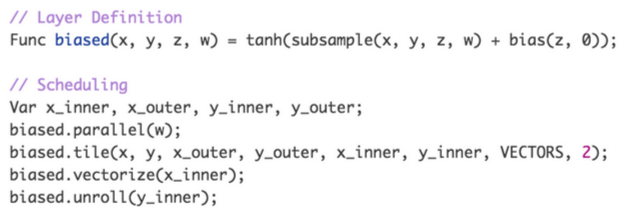
\includegraphics[scale=.7]{halide.png}
\caption{Sample Halide code with algorithm and scheduling separated.}
\end{figure}

Another, less obvious parallelism in our network is on the layer level.
Each layer is only dependent on the layer before it, and within each layer each pixel is completely independent of the other pixels.
Therefore, we can using SIMD vector instructions through the ``\texttt{.vectorize()}" notation, combined with tiling and loop unrolling through the ``\texttt{.tile()}" and ``\texttt{.unroll()}" instructions to improve runtime.
We emperically found that 4-wide vector instructions performed best.

One feature in Halide is it's lazy evaluation.
Halide will only compute the values of a pixel if the final image is dependent on it.
However, as Halide does its computation, it may perform different pieces of different layers out of order.
This means that if certain output pixels are dependent on the same input pixels, there is a chance that it will be computed multiple times.
By using the ``\texttt{.compute\_root()}" notation, we assure that each layer is fully computed before the next layer is started.
While this may seem to hurt computation, because at each pixel at each layer the same amount of work is done, the removal of any repetitive work significantly speeds up our program.

The analysis that led us to all these different routes of parallelism was partly experimental and partly theoretical.  
We experimented with different parameters (such as SIMD widths) very rapidly due to Halide's fantastic design, but actually coming up with each style of parallelism took some deep analysis of the neural network we were designing.
A snippet of this modular approach can be seen in Figure 2.

\section{Results}

We were very happy with our results for the LeNet convolution neural network evaluation times, the results of which are shown in Figures 3 and 4.

We chose not to explore GPU evaluation on the NVIDIA K40 GPUs on the Latedays cluster, as we believed we had a better chance of out-performing Caffe's CPU implementation.  
Additionally, we believe the CPU primitives in Halide allowed us to experiment with a wider variety of parallelism than the GPU scheduling primitives.  
It's possible that our implementation could be competitive with Caffe on the Tesla K40 or another GPU, but that would require a rescheduling of the Halide code, due to Halide having different CPU and GPU primitives.

In order to measure performance, we timed the execution of our Halide implementation using wall-clock time.  
We fed it different amounts of images and averaged over that number to obtain a rate in images per millisecond.  
The inputs were generated by simply choosing a number of images to classify with our code.  
As seen in Figure 3, we achieve a throughput that is within 14\% of Caffe's (using blob size 100).  
The execution behavior of our code on low amounts of work suffers from the heavy set up time that Halide requires to construct the dependency graph of the computation.  
This was confirmed by the shape of our curve in Figure 1, which shows an obvious linear decrease in the small workloads (10, 50, 100).  
This means that the overhead of analyzing the computation is the limiting factor in Halide's execution, since we achieve double the throughput on double the images, i.e. we compute all the images in essentially constant time with respect to the precomputation.  

\begin{figure}
\centering
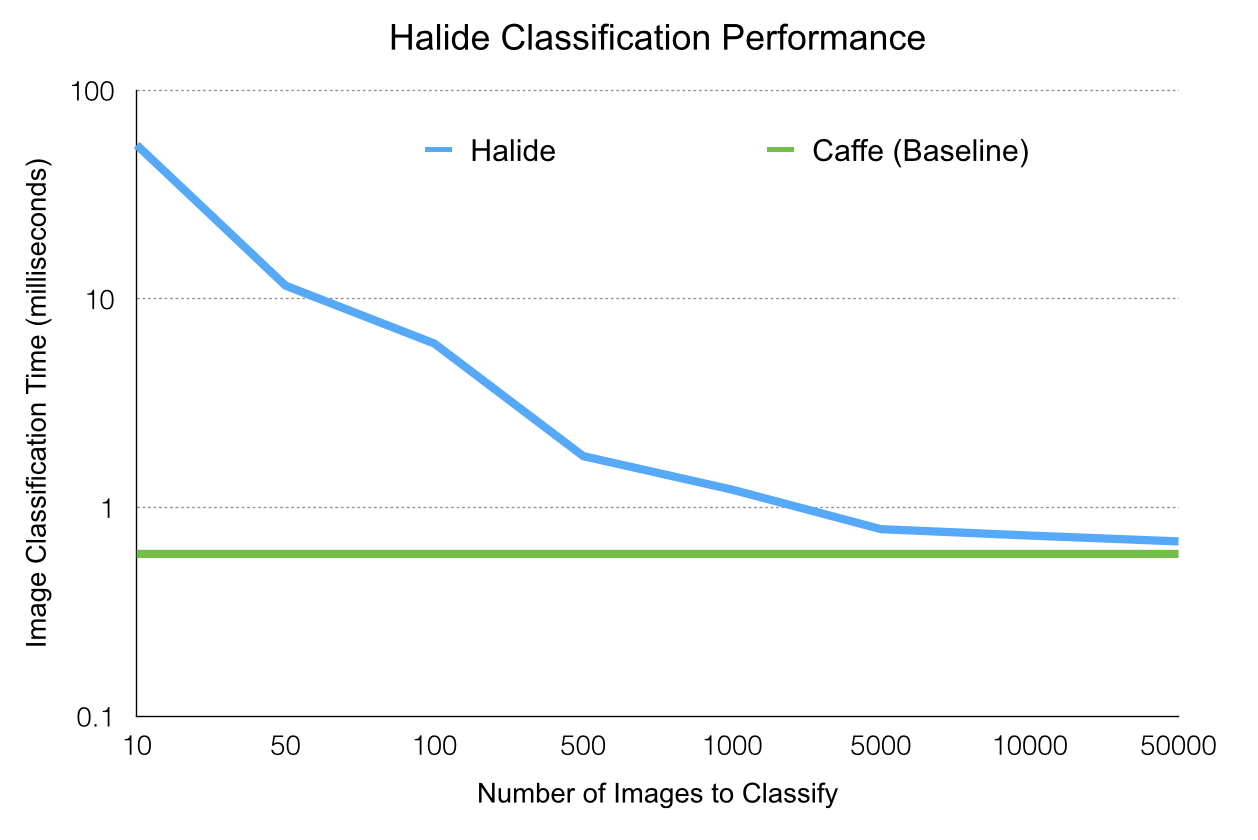
\includegraphics[scale=.5]{graph.png}
\caption{Image throughput (ms/image) versus size of workload (number of images)}
\end{figure}

\begin{figure}
\centering
\begin{tabular}{| c | c |} \hline
Number of Images to Classify & Classification Time (milliseconds / image) \\ \hline
10 & 54.74 \\ \hline
50 & 11.55 \\ \hline
100 & 6.11 \\ \hline
500 & 1.77 \\ \hline
1000 & 1.22 \\ \hline
5000 & 0.79 \\ \hline
10000 & 0.74 \\ \hline
50000 & 0.69 \\ \hline
\end{tabular}
\caption{Halide classification times for different testing set sizes.}
\end{figure}

In terms of a layer by layer analysis, we are doing the most work in the convolution and pooling layers. 
This was confirmed by our analysis during scheduling optimization, where we determined many usual forms of parallelism (like tiling) did not help our fully connected layer reduce execution time.  
We hypothesize that this is because there was not enough work to perform at this layer when compared to the others, so it was not beneficial to set up the thread pool due to the overhead cost.  
The convolution layers and subsampling layers benefited from Halide's scheduling primitives immensely, as we consistently found factors of speedup by adding more sophisticated scheduling during our optimization process.  
We did not formally benchmark the individual components of our pipeline with timing code, but our observations during the development process suggest the above conclusions.

As a final note, we'd like to comment on the plausibility of implementing backpropagation in a Halide pipeline.  It seems like we lose most of the benefit that Halide offers us, because we would almost need to apply ``\texttt{.realize()}" for every layer, since each layer would need to read a different gradient than the final gradient at the lowest layer.  That is to say, during backpropagation our intermediate results are crucial to the algorithm, whereas during forward evaluation we do not care about the values of our image at every layer.  So, there would be no hope of doing any better (or even close to) Caffe's already existing implementation.  However, there is a possibility that we could pipeline this using a similar strategy to the work-efficient parallel \texttt{scan} operation discussed in lecture.  With this methodology we could compute something like a partial gradient at every layer using only what we've computed up to that point, and then allow Halide to communicate between layers (not permitted in usual implementations like Caffe).  This would lead to a pipeline that, at completion, allows every layer to be accessing an image that has the proper gradients for it to read off.  If such a pipeline was possible in Halide we could potentially obtain massive speedup versus what we imagine to be purely sequential Caffe calculation of the gradient during backpropagation.  This is a topic we could explore in the future, should our Halide implementation of forward analysis prove to be competitive even after more robust testing than what we have presented here.

\section{References}

1.  Jonathan Ragan-Kelley, Connelly Barnes, Andrew Adams, Sylvain Paris, Frédo Durand, and Saman Amarasinghe. 2013. Halide: a language and compiler for optimizing parallelism, locality, and recomputation in image processing pipelines. In Proceedings of the 34th ACM SIGPLAN conference on Programming language design and implementation (PLDI '13). ACM, New York, NY, USA, 519-530. DOI=10.1145/2491956.2462176 http://doi.acm.org/10.1145/2491956.2462176

2.  Jia, Yangqing and Shelhamer, Evan and Donahue, Jeff and Karayev, Sergey and Long, Jonathan and Girshick, Ross and Guadarrama, Sergio and Darrell, Trevor.  Caffe: Convolutional Architecture for Fast Feature Embedding.  2014.  arXiv:1408.5093

3.  F. Bastien, P. Lamblin, R. Pascanu, J. Bergstra, I. Goodfellow, A. Bergeron, N. Bouchard, D. Warde-Farley and Y. Bengio. “Theano: new features and speed improvements”. NIPS 2012 deep learning workshop.

\section{Work Distribution}

Implementation of the Halide algorithm was performed by Phil Massey.  
Analysis of Caffe's input structure, modification of the prototext files, and timing tests were performed by Arjun Kar.  
Analysis of Theano's network architecture was performed by Arjun Kar.  
A correctness test of the Halide algorithm versus Theano's implementation was performed by Phil Massey. 
Scheduling of the Halide pipeline was performed by Phil Massey and Arjun Kar.  
The writeup and presentation were prepared by Phil Massey and Arjun Kar.











\end{document}
